\documentclass{beamer}
\usepackage{csquotes}
\usepackage[spanish]{babel}
\usepackage{pgfplots}
\pgfplotsset{width=8cm,compat=1.9}
\usepackage{hyperref}
\usepackage{multirow}
\usepackage{amsmath}
\usepackage{pgfplots}
\usepackage{enumitem}

\usepackage[
backend=biber,
style=authoryear,
sorting=ynt
]{biblatex}

\addbibresource{data_untrm.bib}

\usetheme[sectionstyle=style2]{trigon} % Use trigon theme
\title{Análisis de datos para la investigación}
 
\date {\today}
\author {Andrés Vargas}
\institute {Universidad del Norte \\ Departamento de Economía}
\begin{document}
	\maketitle
\section{Conceptos básicos para el análisis de datos}

\begin{frame}{Propósitos del AD}
Propósito de la actividad científica es explicar (¿Qué es una explicación?). Los datos, y su análisis nos ayudan a explicar, a responder \textit{¿Por qué pasan las cosas como pasan?}
\begin{enumerate}
    \item Datos: representación simbólica. Cuantitativa (medición de observaciones) o cualitativa (texto, imágenes,...)
    \item Información: conocimiento que se obtiene sobre algo
    \item Datos se convierten en información a través del análisis
    \item Contribuyen a explicar a partir de: i) relaciones entre variables, ii) identificación de efectos causales, iii) predicción
\end{enumerate}
    
\end{frame}

\begin{frame}{Datos y métodos de análisis}
Los métodos de análisis adecuados están en función de
\begin{itemize}
    \item La pregunta a responder
    \item El origen de los datos: observacionales, experimentales
    \item El tipo de variables y su relación con el concepto medido
    \begin{itemize}
        \item Cuantitativas: discretas (\# estudiantes en clase), continuas (edad, peso)
        \item Cualitativas: nominales (¿Fuma?: si, no), ordinales (nivel educativo: primaria, secundaria, universitario)
    \end{itemize}
\end{itemize}
    
\end{frame}

\begin{frame}{Causalidad y predicción}

Ejemplos

\begin{enumerate}
    \item El modelo indica que la sustancia A es mejor para anestesiar ratones que la sustancia B: exponer ratones a las dos sustancias y comparar las respuestas fisiológicas. Si el modelo es creíble entonces debe haber diferencia en la respuesta biológica. Todos los demás factores que pueden afectar la respuesta fisiológica han sido tenidos en cuenta
    \item Cuáles son los factores que influencian la diversidad de aves en un fragmento de bosque. Tenemos una lista de influencias potenciales ¿Cuál es la combinación que mejor predice la diversidad de aves?
\end{enumerate}
    
\end{frame}

\begin{frame}{Ruido y señal}

El análisis de datos es un ejercicio estadístico. Los datos tienen ruido y señal ¿Cómo separamos?

\begin{itemize}
    \item Señal: información que intentamos detectar
    \item Ruido: variabilidad no deseada que interfiere con la señal
\end{itemize}

¿El dinero nos hace felices? La gente más adinerada también pueden tener mejor trabajo, un mejor estatus social, ..., otros factores que también la hacen más felices. Por lo tanto, la correlación entre ingreso y felicidad es ruidosa
    
\end{frame}

\begin{frame}{Podemos obtener conclusiones erróneas}

\begin{itemize}
    \item No hay correspondencia entre la pregunta de interés y el diseño experimental o la fuente de datos utilizados (quiere saber si las mujeres tienen una respuesta mayor que los hombres a un tratamiento médico, pero el diseño del experimento no tuvo en cuenta el sexo)
    \item El modelo estadístico no está relacionado con el modelo teórico
    \item Los datos no son confiables: mal diseño o ejecución del experimento, muestreo inadecuado,...
    \item No se cumplen los supuestos del modelo estadístico: normalidad, ...
    \item Presión por obtener resultados significativos
\end{itemize}
    
\end{frame}

\begin{frame}{Ejercicio}

Revise cada uno de los artículos siguientes \cite{low_mouse} y \cite{loyn1987effects} y establezca la relación entre la pregunta de investigación, el método de recolección de datos, y el método de análisis de datos. Para ello

\begin{enumerate}
    \item Identifique la pregunta/objetivo de investigación ¿Busca establecer una relación causa-efecto o una predicción?
    \item ¿Los datos son observacionales o experimentales? Describa como se obtuvieron los datos
    \item ¿Cuál es el tipo de cada una de las variables utilizadas? (cuantitativa,...)
    \item ¿Cómo se analizaron los datos? Distinga entre la variable dependiente y las independientes 
    \item ¿Cuál es la conclusión que se deriva del análisis de datos?
\end{enumerate}
    
\end{frame}

\begin{frame}{La \textit{Lógica experimental}}

Un experimento no es otra cosa que la variación \textit{deliberada} y \textit{controlada} de una variable para averiguar la respuesta de una variable de resultado. Nos interesa la \textbf{existencia} del efecto así como su \textbf{magnitud}

\begin{itemize}
    \item Observacionales: nos basamos en modelos estadísticos, técnicas de estimación e identificación de efectos. Muy común en economía y otras ciencias sociales
    \item Experimentales: aislar otros factores, determinar la capacidad de detectar el efecto
\end{itemize}
    
\end{frame}

\begin{frame}{Planeación e implementación}

\begin{itemize}
    \item Definir el objetivo
    \item Elegir la variable de respuesta: tipo de variable, capacidad para medirla bien
    \item Factores y niveles: los factores son las variables que se varían deliberadamente, los niveles son los valores que puede tomar el factor. Por ejemplo, $T=1$ si toma la píldora y $T=0$ si no toma la píldora. Un tratamiento es la combinación de factores y niveles. $M=1$ si es mujer y $M=0$ si no es mujer, entonces $T=1$ y $M=0$ es un tratamiento
    \item Plan experimental
    \item Ejecución
    \item Análisis de datos
    \item Conclusiones
\end{itemize}
    
\end{frame}

\begin{frame}{Principios de la experimentación}

\begin{enumerate}
    \item Replicación: cada tratamiento es aplicado a unidades experimentales que son representativas de la población. Tamaño de muestra afecta la incertidumbre de las estimaciones y el poder de la prueba. Replicación $\neq$ repetición
    \item Aleatorización: asignación de unidades a los tratamientos, el orden en el que se aplican los tratamientos, el orden en el que las respuestas son medidas. Evita la influencia de variables no observadas, asegura la validez de la estimación del error que se usa para la inferencia
    \item Bloqueo: agrupación de unidades homogéneas entre si. 
    

\end{enumerate}
    
\end{frame}

\begin{frame}{El modelo de regresión lineal}


El gobierno implementa un programa de nutrición infantil en el que le entrega a los niños un complemento alimenticio. Quiere saber el efecto del programa. Su variable de resultado es un indicador de desnutrición aguda, $Y=Peso/Talla$. Sea $X=1$ si el niño estuvo en el programa y $X=0$ si el niño no estuvo en el programa. Expresamos la relación entre la desnutrición y la participación en el programa, $j$, para el niño $i$ como

\begin{equation*}
    Y_{ij}=\beta_0+\beta_1X_{ij}+\varepsilon_{ij}
\end{equation*}

    
\end{frame}

\begin{frame}{El modelo de regresión lineal}

\begin{equation*}
    Y_{i}=\beta_0+\beta_1X_i+\varepsilon_i
\end{equation*}

El estado nutricional de un niño está en función de la participación en el programa y un término de error. 

\begin{enumerate}
    \item $Y_{ij}$: variable de respuesta. Continua
    \item $X_{ij}$: factor, 2 niveles $(1,0)$. Categórica, nominal
    \item $\varepsilon_{ij}$: error
    \item $\beta_0$ y $\beta_1$: parámetros
\end{enumerate}
    
\end{frame}

\begin{frame}{El modelo de regresión lineal}

\begin{itemize}
    \item Nuestros datos son observaciones, $Y_{ij}$ y $X_{ij}$
    \item Son una muestra de muchas posibles: variabilidad muestral
    \item ¿Cómo se seleccionaron los datos que conforman la muestra?: ¿Aleatorización?
    \item ¿Es el tamaño de la muestra suficiente para detectar el efecto?: poder
\end{itemize}
    
\end{frame}

\begin{frame}{El modelo de regresión lineal}

Los parámetros $\beta_0$, $\beta_1$ capturan la relación entre los factores y $X$

\begin{itemize}
    \item Son desconocidos. Los estimamos a partir de la muestra
    \item Incertidumbre/precisión en su estimación: producto de la variabilidad muestral
    \item Relación: ¿Correlación o efecto causal? Depende de su relación con el error $\varepsilon$
\end{itemize}
    
\end{frame}

\begin{frame}{El modelo de regresión lineal}
    El término de error recoge todo lo demás que afecta el estado nutricional y variación completamente aleatoria. Si no hay relación entre $\varepsilon$ y $X$ (lo desarrollaremos más adelante), entonces este modelo nos permite recoger el efecto de $X$ sobre $Y$
\end{frame}

\begin{frame}{El modelo de regresión lineal}

\begin{equation*}
    Y_{i}=\beta_0+\beta_1X_i+\varepsilon_i
\end{equation*}

¿Cómo nos aseguramos de que no haya relación entre $\varepsilon$ y $X$?

\begin{itemize}
    \item Datos experimentales: diseño experimental
    \item Datos observacionales: no puede. Intenta identificar el efecto a través de otros métodos de estimación. Aprovecha situaciones que producen experimentos naturales
\end{itemize}
    
\end{frame}


\begin{frame}{El modelo de regresión lineal}

Volviendo a nuestro ejemplo ¿Cómo sabemos si el programa funcionó? Comparamos el estado nutricional promedio de quienes participaron, $\bar{Y_1}$ con el de quienes no participaron, $\bar{Y_0}$, donde

\begin{equation*}
    \bar{Y_j}=\dfrac{1}{n_j}\sum_iY_{ij}
\end{equation*}
 \begin{itemize}
     \item $H_0:\bar{Y_1}-\bar{Y_0}=0$; $H_a:\bar{Y_1}-\bar{Y_0}\neq 0$
     \item Para saber si son diferentes los promedios debemos asegurarnos de que no es simple chance. Recuerde la variabilidad muestral
 \end{itemize}
     
\end{frame}

\begin{frame}{Modelo de regresión}
Si los promedios son diferentes, ¿esto es debido a $X$? ¿Podrían ser otras factores?

\begin{align*}
    E(Y_{ij}|T_{ij}=0)&=\beta_0+E(\varepsilon_{ij}|T_{ij}=0)\\
    E(Y_{ij}|T_{ij}=1)&=\beta_0+\beta_1+E(\varepsilon_{ij}|T_{ij}=1)\\
    \end{align*}

    Luego

    \begin{equation*}
        E(Y_{ij}|T_{ij}=1)-E(Y_{ij}|T_{ij}=0)=\beta_1+E(\varepsilon_{ij}|T_{ij}=1)-E(\varepsilon_{ij}|T_{ij}=0)
    \end{equation*}

\end{frame}

\begin{frame}
    El promedio es un estimador del valor esperado, luego

    \begin{align*}
        \bar{Y}_0&=\hat{\beta}_0\\
        \bar{Y}_1&=\hat{\beta}_0+\hat{\beta}_1
    \end{align*}  

    Por lo tanto 

    \begin{equation*}
        \bar{Y}_1-\bar{Y}_0=\hat{\beta}_1
    \end{equation*}
    Y 
    \begin{equation*}
        \hat{\beta}_1=\beta_1 \quad \text{si}\quad E(\varepsilon_{ij}|T_{ij}=1)=E(\varepsilon_{ij}|T_{ij}=0)
    \end{equation*}

    El estimador corresponde al efecto causal, la diferencia en $Y$ atribuible únicamente a $X$, si no hay relación entre el error y $X$
\end{frame}

\begin{frame}{Recapitulando}

\begin{enumerate}
    \item Para explicar nos interesa capturar la relación causa-efecto entre $X$ y $Y$
    \item Estadísticamente esto requiere que eliminemos las potenciales fuentes de relación entre el error y $X$. Esto es lo que buscamos lograr con el diseño experimental. Justifica el análisis de regresión y ANOVA
    \item Con datos observacionales necesitamos otras estrategias (no es tema de este curso)
\end{enumerate}
    
\end{frame}

\section{Estadística inferencial y análisis de datos}

\begin{frame}{Definición}

Es el conjunto de métodos para inducir a partir de una muestra el comportamiento de una población. Inferir las propiedades de una distribución de probabilidad subyacente

\begin{itemize}
    \item Muestra: colección de observaciones de una población
    \item Estadísticas: características de la muestra (promedio, $\hat{\beta}$)
    \item Características de la población: parámetros (media poblacional/valor esperado, $\beta$)
    \item Muestra aleatoria: cada observación tiene la misma probabilidad de ser incluida en la muestra
\end{itemize}
    
\end{frame}

\begin{frame}{Variabilidad muestral}

Tomamos 2 muestras de tamaño n de una población de tamaño N. Para cada muestra calculamos el promedio de la variable $Y$. Con seguridad serán diferentes, ¿Por qué?

\begin{itemize}
    \item Variabilidad natural entre los individuos
    \item Error de medición: instrumentos de medición imperfecto
\end{itemize}

    Realice el ejercicio de simulación simul1.R
\end{frame}

\begin{frame}{Probabilidad \footnote{Se recomienda este \href{https://www.probabilitycourse.com/chapter1/1_1_0_what_is_probability.php}{\textcolor{blue}{texto}}}}

\begin{itemize}
    \item Aleatoriedad e incertidumbre: nuestro conocimiento sobre el resultado es limitado, por lo tanto no sabemos con certeza qeu pasará
    \item Frecuencia relativa: por ejemplo, si lanzo una moneda el número total de veces que sale cara sobre el total de lanzamientos
    \item Creencia subjetiva: cuantificación de lo que creemos que pasará
    \item Axiomas de probabilidad
\end{itemize}
    
\end{frame}

\begin{frame}{Probabilidad}

Antes de ejecutar un experimento, (ej. lanzar un dado) no conocemos el resultado. Después de ejecutarlo conocemos su resultado. El conjunto de todos los resultados posibles es el espacio muestral

\begin{itemize}
    \item Lanzar una moneda una vez: $S=\{H,T\}$
    \item Lanzar una moneda dos veces: $S=\{(H,H),(H,T),(T,H),(T,T)\}$
    \item Evento: un subconjunto del espacio muestral
    \item El propósito es asignar una probabilidad a ciertos eventos
\end{itemize}
    
\end{frame}

\begin{frame}{Probabilidad}

Axiomas. Decimos que $P(A)$ es una medida de probabilidad del evento A

\begin{enumerate}
    \item Axioma 1: Para cualquier evento A, $P(A)\geq 0$
    \item Axioma 2: La probabilidad del espacio muestral $S$ es $P(S)=1$
    \item Axioma 3: Si $A_1,A_2,...$ son eventos mutuamente excluyentes, entonces $P(A_1\cup A_2 \cup A_3...)=P(A_1)+P(A_2)+P(A_3)+... $
\end{enumerate}
    
\end{frame}

\begin{frame}{Probabilidad condicional}

Probabilidad de la ocurrencia de un evento dada la ocurrencia de otro evento. Otra manera de verlo, en la medida que obtenemos más información, ¿cómo actualizamos la probabilidad del evento de interés?

Si el 23\% de los días son lluviosos, entonces $P(R)=0.23$. Si le digo que el día está nublado ¿Cuál es la probabilidad de lluvia en este día? $P(R|C)$ donde $C$ significa que está nublado. De manera general, si $A$ y $B$ son dos eventos, entonces

\begin{equation*}
    P(A|B)=\dfrac{P(A\cap B)}{P(B)}
\end{equation*}
\end{frame}

\begin{frame}{Probabilidad condicional}
    Lanzo un dado. Definimos el evento $A$ como la ocurrencia de un número impar, $A=\{1,3,5\}$. Sea el evento $B$ la ocurrencia de un número menor o igual a 3, $B=\{1,2,3\}$

    \begin{itemize}
        \item $P(A)=\dfrac{|A|}{|S|}=\dfrac{3}{6}=\dfrac{1}{2}$
        \item $P(B)=\dfrac{|B|}{|S|}=\dfrac{3}{6}=\dfrac{1}{2}$
        \item $P(A\cap B)=\dfrac{|A|\cap |B|}{|S|}=\dfrac{1}{3}$
        \item $P(A|B)=\dfrac{2}{3}$
    \end{itemize}
\end{frame}

\begin{frame}{Probabilidad condicional}

Dos eventos son independientes si uno no contiene información sobre el otro
\vspace{2mm}
\begin{block}{Independencia}
Dos eventos A y B son independientes si $P(A\cap B)=P(A)P(B)$
\end{block}

Por lo tanto $P(A|B)=P(A)$
  
\end{frame}

\begin{frame}{Variable aleatoria}

Una variable aleatoria es una función de valor real que asigna un valor numérico a cada resultado posible de un experimento (proceso por el cual observamos algo incierto). Por ejemplo, si lanzo una moneda y defino la variable $X=1$ si la moneda cae en cara y $X=0$ si no cae en cara

\vspace{2mm}

\begin{block}{Variable aleatoria}
Una variable aleatoria $X$ es una función del espacio muestral, $S$, a los números reales
$X:S\rightarrow \mathbb{R}$
    
\end{block}
    
\end{frame}

\begin{frame}{Distribución de probabilidad}

Es una función que describe las probabilidades de sus valores posibles. Para variables discretas comprende las probabilidades medibles para cada resultado posible. Las variables continuas no están restringidas a un valor determinado, luego hay infinitos resultados posibles. Para variables continuas hablas de la probabilidad de un rango dado de valores
    
\end{frame}

\begin{frame}{DP: Variables discretas}

Si $X$ es una variable discreta con rango $R_x=\{x_1,x_2,...,x_k\}$, entonces las probabilidades de eventos particulares está descrita por la función de masa de probabilidad (PMF)

\begin{equation*}
    P_X(x_k)=P(X=x_k), \quad \text{para} \quad k=1,2,3,...
\end{equation*}

Lanzo una moneda dos veces. Sea $X$ el número de caras que se observan. El espacio muestral es $S=\{(H,H),(H,T),(T,T),(T,H)\}$, luego $R_X=\{0,1,2\}$, y la función de probabilidad 
\begin{equation*}
P_X(0)=\dfrac{1}{4}; \quad P_X(1)=\dfrac{1}{4}+\dfrac{1}{4}=\dfrac{1}{2}; \quad P_X(2)=\dfrac{1}{4}    
\end{equation*}

\end{frame}

\begin{frame}{DP: Variable discreta}
\begin{tikzpicture}
\begin{axis}[
ybar,
    title={Función de probabilidad},
    xlabel={$x$},
    ylabel={$P_X(x)$},
    xmin=-1, xmax=3,
    ymin=0, ymax=1,
    xtick={0,1,2},
    ytick={0.25,0.5,0.75,1},
    ]
\addplot[
    color=red,
    mark=square,
    ]
    coordinates {
    (0,0.25)(1,0.5)(2,0.25)
    };
\end{axis}
\end{tikzpicture}
    
\end{frame}
\begin{frame}{Algunas distribuciones discretas}

Sea $X$ una variable aleatoria discreta tal que toma el valor de $1$ si se cumple una condición y $0$ si no se cumple

\begin{block}{Bernoulli}
    Una variable $X$ tiene una distribución de Bernoulli con el parámetro $p$ si su PMF restá dada por
    \begin{equation*}
    P_X(x)=
        \begin{cases}
p \quad \text{si} \quad x=1\\
1-p \quad \text{si} \quad x=0\\
0 \quad \text{en otro caso}
        \end{cases}
    \end{equation*}
\end{block}
    
\end{frame}

\begin{frame}{Algunas distribuciones discretas}

La distribución de Bernoulli es muy útil cuando nuestro estudio analiza variables que capturan la presencia o ausencia de algo. Por ejemplo, los animales viven o mueren, cierta especie está presente o ausente en el bosque, el individuo tomó el bus para ir al trabajo o no tomó el bus para ir al trabajo,...
    
\end{frame}

\begin{frame}{Algunas distribuciones discretas}

La distribución de probabilidad del número de \textit{éxitos} en $n$ ensayos independientes de Bernoulli se llama una distribución binomial

\begin{block}{Bernoulli}
    Una variable $X$ tiene una distribución de Binomial con parámetros $p$ y $n$ si su PMF restá dada por
    \begin{equation*}
    P_X(k)=
        \begin{cases}
        \binom{n}{k}p^k(1-p)^{n-k} \quad \text{para}\quad k=0,1,2,...,n\\
        0 \quad \text{en otro caso}
        \end{cases}
    \end{equation*}
\end{block}
    
\end{frame}

\begin{frame}{Función de de distribución acumulada}

La CDF de la variable aleatoria $X$ se define como 
\begin{block}{CDF}
\begin{equation*}
F_X(x)=P(X\leq x)    \quad \text{para todo} \quad x\in \mathbb{R}
\end{equation*}
    
\end{block}

Si tenemos la PMF, podemos hallar la CDF como

\begin{equation*}
    F_X(x)=\sum_{x_k\leq x}P_X(x_k)
\end{equation*}
    
\end{frame}

\begin{frame}{Valor esperado}

\begin{block}{Valor esperado}
    Sea $X$ una variable aleatoria discreta con rango $R_X=\{x_1,x_2,...\}$. El valor esperado es

    \begin{equation*}
        E(X)=\sum_{x_k\in R_x}x_kP(x_k)
    \end{equation*}
\end{block}
    
\end{frame}

\begin{frame}{Varianza}

\begin{block}{Varianza}
La varianza de la variable aleatoria $X$ con media $E(X)=\mu_X$ es

\begin{equation*}
    Var(X)=E[(X-\mu_X)^2]
\end{equation*}
    
\end{block}

    Se puede mostrar que

    \begin{equation*}
        Var(X)=E(X^2)-\mu^2_X
    \end{equation*}
\end{frame}

\begin{frame}{Variable aleatoria continua}

\begin{block}{Variable aleatoria continua}
    Decimos que la variable aleatoria $X$ es continua si su CDF $F_X(x)$ es una función continua para todo $x \in \mathbb{R}$
\end{block}

Los valores de la variable caen sobre la recta real. Como hay un número infinito de puntos sobre la recta real, aún dentro de un intervalo, la probabilidad de observar un valor particular es cero. Por eso no hablamos de la PMF
    
\end{frame}

\begin{frame}{Variable aleatoria continua: pdf}
    Indica la probabilidad de que la variable aleatoria caiga dentro de un rango determinado de valores

    \begin{block}{pdf}
    Una variable aleatoria $X$ con CDF absolutamente continua $F_X(x)$. La función $f_X(x)$ se define como

    \begin{equation*}
        f_X(x)=\dfrac{dF_X(x)}{dx}=F_X'(x), \quad \text{si es diferenciable en} \quad x 
    \end{equation*}
        
    \end{block}

    Como la pdf es la derivada de la CDF, entonces

    \begin{equation*}
        F_X(x)=\int_{-\infty}^x f_X(u) \, du
    \end{equation*}
\end{frame}

\begin{frame}{Variable aleatoria continua}

Considere la variable aleatoria continua $X$ cuya pf está dada por

\begin{equation*}
    f_X(x)=
    \begin{cases}
        e^{-x} \quad \text{si} \quad x\geq 0\\
        0 \quad \text{en otro caso}
    \end{cases}
\end{equation*}

De donde 

\begin{equation*}
    F_X(x)=
    \begin{cases}
        1-e^{-x} \quad \text{si} \quad x\geq 0\\
        0 \quad \text{en otro caso}
    \end{cases}
\end{equation*}

En una hoja de excel grafique ambas funciones para valores de $X$ en el intervalo $[0,4]$ usando incrementos de 0.1 unidades. Halle la probabilidad de $1<X<3$
    
\end{frame}

\begin{frame}{Valor esperado}

En el caso de una variable aleatoria continua, el valor esperado está dado por

\begin{equation*}
    E(X)=\int_{-\infty}^{\infty}xf_X(x)dx
\end{equation*}
    
\end{frame}

\begin{frame}{Distribución Normal}

Si $X$ es una variable aleatoria con distribución normal con media $\mu$ y varianza $\sigma^2$, $X\sim N(\mu,\sigma^2)$, entonces

\begin{equation*}
    f_X(x)=\dfrac{1}{\sigma\sqrt{2\pi}}exp\left\{-\dfrac{(x-\mu)^2}{2\sigma^2}\right\}
\end{equation*}
    
\end{frame}

\begin{frame}{Otras distribuciones}

Para pruebas estadísticas, solemos usar las siguientes distribuciones

\begin{itemize}
\small{
    \item $z$ o normal estándar: pdf de una variable aleatoria $N(0,1)$. Es el la razón entre la difrencia de la estadística muestral con su valor poblacional y la desviación estándar poblacional
    \item $t$ de student: probabilidad de una variable aleatoria que es la razón de la diferencia entre la estadística muestral con su valor poblacional y la desviación estándar muestral. Test de medias, hipótesis sobre los parámetros individuales en un modelo de regresión
    \item $\chi ^2$ es la distribución de una variable que es el cuadrado de los valores de una distribución normal estándar. No puede ser negativa. Las varianzas tienen esta distribución
    \item $F$ representa la distribución de probabilidad de una variable que es la razón de dos $\chi ^2$ independientes, cada una dividida por sus grados de libertad. Comparar varianzas. ANOVA y pruebas de significancia conjunta de parámetros en un modelo de regresión lineal
    }
\end{itemize}
    
\end{frame}

\begin{frame}{Otras distribuciones}

\begin{figure}
\centering
        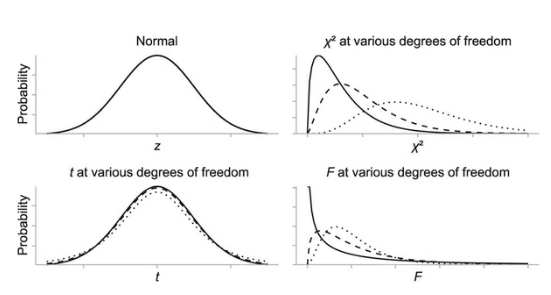
\includegraphics[scale=0.8]{distribuciones.PNG}
        
        \end{figure}
    
\end{frame}

\begin{frame}{Pruebas de hipótesis}

Ya tenemos los ingredientes para hacer pruebas

\begin{enumerate}
    \item Queremos averiguar algo sobe la población. Hipótesis
    \item Para ello usamos una muestra
    \item Con esa muestra estimamos el valor poblacional
    \item Pero, si hubiésemos tenido otra muestra, nuestra estimación sería diferente. Variabilidad muestral
    \item El estimador entonces es una variable aleatoria
    \item Por lo tanto está caracterizado por una función de distribución
    \item En consecuencia, nuestra estimación estará a alguna distancia del valor poblacional de acuerdo a la hipótesis
    \item Necesito una regla para decidir si el valor estimado es consistente con la hipótesis
\end{enumerate}
    
\end{frame}

\begin{frame}{Pruebas de hipótesis}

Para decidir si es consistente necesitamos un criterio

\begin{itemize}
    \item Distancia entre el valor estimado y el de la hipótesis
    \item Debemos tener en cuenta la variabilidad del estimador: desviación estándar del estimador
    \item ¿La desviación que observamos cómo es en relación a la desviación típica?
\end{itemize}
    
\end{frame}

\begin{frame}{Prueba de hipótesis: ejemplo}
    Recuerde nuestro ejercicio de simulación. Tome una muestra cualquiera de tamaño 30 de la población. Calcule el promedio. Para esa muestra obtuve $\bar{y}=166.6$. Este es un valor estimado de la media poblacional, $E(Y)$
    \begin{enumerate}
        \item $H_0:E(Y)=165$ Hipótesis: la media poblacional de Y es 165. ¿Es el valor estimado consistente con esa hipótesis del valor poblacional?
        \item Distancia entre el estimado y la la hipótesis: $164.6-165$
        \item Debido a la variabilidad muestral puede haber obtenido otros promedios. Desviación estándar del promedio estimado con todas las muestras posibles de tamaño $n$. No lo conocemos, pero lo estimamos. Error estándar
        \item $s.e(\bar{y})=sd(y)/\sqrt{n}=2.529$
    \end{enumerate}
\end{frame}

\begin{frame}{Prueba de hipótesis: ejemplo}
    \begin{enumerate}[start=5]
        \item Razón entre la distancia y la desviación: $\dfrac{\bar{y}-E(Y)_{H_O}}{s.e(\bar{y})}=\dfrac{164.6-165}{2.529}=-0.146$
        \item La desviación observada respecto a la hipótesis es -0.14 veces la desviación estándar (estimada) del estimador
        \item Se distribuye como una $t$ de student
        \item Para poder saber si es consistente con la hipótesis, necesitamos una hipótesis alternativa. 
    \end{enumerate}
\end{frame}

\begin{frame}{Prueba de hipótesis: ejemplo}

\begin{enumerate}[start=9]
    \item Defino $H_1:E(Y)\neq 165$. Puede haber definido que era mayor o menor. 
    \item Para una distribución $t$ con 29 grados de libertad el 95\% de las observaciones está entre -2.045 y 2.045. El 95\% de las muestras arrojaría un valor en dicho intervalo
    \item Mi valor estimado y por lo tanto el $t$ calculado está dentro del 95\%. No es raro que haya encontrado este valor
\end{enumerate}
    
\end{frame}

\begin{frame}{Prueba de hipótesis: ejemplo}

\begin{itemize}
    \item Si la hipótesis nula es correcta, $H_0=165$, entonces mi estadística $t$ debe estar dentro de este intervalo del 95\% (nota: puede haber definido un intervalo diferente)
    \item Si mi estadística cae por fuera de dicho intervalo, entonces mis datos rechazan la $H_0$ a favor de $H_1$
    \item En este caso, como $t leg|t_c|$ entonces no rechazo la hipótesis
    \item Conclusión: mi valor estimado, 164.6, no es estadísticamente diferente de 165
    \item Repita el ejemplo pero ahora use un tamaño de muestra $n=10$ ¿Se mantiene la conclusión?
\end{itemize}
    
\end{frame}

\begin{frame}{Prueba de hipótesis: errores}

La mayoría de las veces comparamos la media de la variable de resultado para diferentes grupos. En ese caso formulamos la hipótesis nula, por ejemplo para dos grupos, como $H_0: \bar{y}_1-\bar{y}_2=0$. Por ejemplo, en el caso del paper de \cite{low_mouse} nos interesa la diferencia en la respuesta fisiológica entre los que se les administra la sustancia Isoflurane, $I$ y los que reciben Alpha Chloralose, $A$. Sea la variable de respuesta la tasa de respiración, entonces la hipótesis es

\begin{align*}
    H_0:& \bar{y}_I-\bar{y}_A=0\\
    H_1:& \bar{y}_I-\bar{y}_A \neq 0
\end{align*}
    
\end{frame}

\begin{frame}{Prueba de hipótesis: errores}

Lo anterior lo puedo reformular de la siguiente manera. Definimos la variable $T=1$ si se le administró la sustancia $I$ y $T=0$ si se le administró la sustancia $A$

\begin{equation*}
    y_i=\alpha+\beta T+ e
\end{equation*}

De acá, podemos mostrar que $\bar{y}_I=\hat{\alpha}+\hat{\beta}$,  y $\bar{y}_A=\hat{\alpha}$, luego $\bar{y}_I-\bar{y}_A=\hat{\beta}$. De donde

\begin{equation*}
    H_0:\beta=0
\end{equation*}
    Si los datos soportan la hipótesis, digo que no hay efecto, que el coeficiente no es significativo. Si rechazan la hipótesis, hay evidencia de efecto, coeficiente significativo.
\end{frame}

\begin{frame}{Prueba de hipótesis: errores}

Nuestra conclusión puede ser errada, en relación con la situación real

\begin{figure}
\centering
        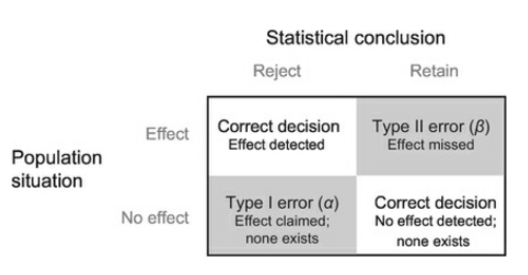
\includegraphics[scale=0.8]{error.PNG}
        
        \end{figure}
    
\end{frame}

\begin{frame}{Prueba de hipótesis: significancia}

En nuestro ejemplo elegimos el intervalo de 95\%. Por fuera de ese intervalo está el 5\%, a este lo llamamos $\alpha$
\begin{itemize}
    \item $\alpha$: nivel de significancia. Probabilidad de rechazar la hipótesis nula cuando es cierta. Si $\alpha=0.05$, solo el 5\% de las muestras posibles arrojaría un valor por fuera del intervalo del 95\% del estadístico. Si el estadístico que obtengo, esta por fuera de dicho intervalo, entonces la probabilidad de rechazar la nula siendo correcta es inferior al 5\%
    \item Nivel de confianza: $1-\alpha$
\end{itemize}
    
\end{frame}

\begin{frame}{Prueba de hipótesis: p-value}

La probabilidad de obtener un valor tan o más extremo al observado si la hipótesis nula es cierta. Si el estadístico tienen un valor grande quiere decir que estamos en la cola de la distribución, en consecuencia la probabilidad de obtener esos valores es pequeña
\begin{figure}
\centering
        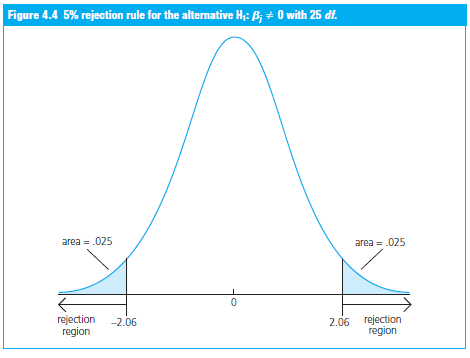
\includegraphics[scale=0.5]{twotailed.PNG}
        
        \end{figure}

    
\end{frame}

\printbibliography

\end{document}
